
\chapter{基于标签同步解码的搜索空间优化}
\label{chap:lsd}

本论文基于端到端建模,系统地提出了标签同步算法,其通过一系列方法使得搜索解码过程从逐帧同步变为标签同步,从而加速解码。

为了对语音识别中的时序特征进行建模,人们提出了序列模型。根据其建模过程,序列模型包含GSM和DSM,在第\ref{Sec:seq-tr-review}章节进行了介绍。
通常来说,出于以下原因,GSM和DSM被分解为帧层面的训练准则:1)为了更加高效地发挥帧层面分类器的建模效果,如混合高斯模型(Gaussian mixture model, GMM~\cite{woodland1994large})和深度神经网络(deep neural network, DNN ~\cite{hinton2012deep});2)为了减轻模型的稀疏性,以及通过将简单模型分解为多个组分来增强模型的泛化能力,例如ASR中将模型分解为声学模型、字典和语言模型等;3)未经序列分解的模型在推理搜索前需要得到整个序列信息进而进行后续处理,这将给解码过程造成严重的运行延时。本文提出的序列标注方法即是基于帧层面分解的模型~\cite{forney1973viterbi,mohri2002weighted}。

在推理搜索阶段,为了找到与输入特征最为匹配的标签序列,搜索过程需要将声学模型,语言模型和字典等模型结合起来。该过程是通过在每帧使用基于束剪枝的维特比算法来实现的~\cite{forney1973viterbi},称为帧同步解码(frame synchronous decoding, FSD)。在该框架中,我们将特征帧的数量和语句长度的比值定义为特征速率,将标签输出数量与语句长度的比值定义为标注速率,将解码的帧数与语句长度的比值定义为解码速率。那么,在帧同步解码中,这三个速率均相等。

虽然已经被广泛使用,但帧同步解码仍存在一些缺点:1)这是一个等间隔搜索算法,在处理可变长序列时较为低效。2)由于序列被分解为帧来作为特征序列,模型的粒度变小,导致搜索空间很大。比如ASR中词语历史,音素序列,以及HMM状态之间的关联性通常以加权有限状态机(weighted finite-state transducer, WFST)进行表示(通常称为HCLG~\cite{mohri2002weighted} 搜索空间)。由于由多个庞大知识源共同组成,因此组成该搜索空间的状态机最终达到百亿条边。3)在每帧进行贪心束剪枝通常很难兼顾搜索效率和搜索误差。

如第~\ref{chap:intro2-dec-todo}章节中对于解码搜索的研究机遇的讨论,近来神经网络的发展使得更强的上下文和历史建模效果成为可能\cite{sak2014long,qian2016very}。同时,更多的标注数据也进一步缓解了模型的稀疏性和泛化问题。这些进展使得研究人员们有可能在更大的模型粒度上-从帧到整个序列层面~\cite{amodei2015deep,soltau2016neural,collobert2016wav2letter,sak2015fast,chan2016end}进行序列分解,如Soltau等人报道的一个基于单词粒度深度学习的声学模型\cite{soltau2016neural},在125K小时标注数据上的表现优于较小粒度的模型。在这些研究中,标注速率小于特征速率,但解码速率仍然等于特征速率。

本文提出将特征层面的搜索过程改变为标签层面,即搜索空间是由不同历史的标签组成的,使得解码速率等于标注速率,从而小于特征速率。具体来说,在标签推理搜索阶段,对帧层面声学模型的输出增加一步后处理过程:i)判断当前帧是否存在标签输出;ii)若有,执行搜索过程;若无,则丢弃标签输出。因此该后处理过程可被看作是每个输出标签概率计算的近似。与传统方法相比,该方法的优势是搜索空间更小,且搜索过程被大大加速。
该文提出的一系列通用方法在隐马尔科夫模型和连接时序分类模型上得到了验证。

最终在实验部分,该章节系统取得大幅度语音识别解码速度改善。

\section{基于连接时序分类模型的标签同步解码}
\label{chap:lsd-ctc}

我们在第\ref{Sec:sgm-and-sdm}章节总结了语音识别中的序列建模方法。在模型推理搜索阶段,为了找到与输入特征最为匹配的标签序列,搜索过程需要将前述序列模型与其它知识源,即字典、语言模型等融合起来。即解码标签序列是由前述各分解序列所共同决定的。该搜索过程是通过在每帧上使用基于束剪枝的维特比算法进行的\cite{forney1973viterbi},即第\ref{chap:lsd-review-fsd}章节介绍的传统帧同步解码算法。该框架中,解码速率等于标注速率,标注速率等于特征速率。

尽管被广泛使用,FSD方法仍有一些缺点:1)它是一个等间隔搜索算法,处理变长特征序列较为低效。即使在采用第\ref{chap:intro2-score}章节总结的跳帧等分数计算优化算法时仍存在该问题。 2)当序列被分解为帧层面作为特征序列时,模型粒度较小,导致搜索空间很大。3)在每帧均进行贪心束剪枝,很难平衡搜索效率和搜索误差。因此,本文通过将特征层面的搜索过程改变为标签层面,提出了基于端到端建模的标签同步推理搜索,接下来作者将对该框架及其应用进行详细介绍。


该部分中,本文提出将搜索过程从特征层面改为标签层面,称为标签同步解码(label synchronous decoding, LSD)。本部分将对DSM中的LSD进行公式推导,具体实现方案及一些解码加速的经验方案也将进行讨论。

\subsection{标签同步解码}
\label{chap:lsd-lsd-ctc-method}
在测试阶段,在基于音素的CTC模型中,从公式 \ref{eq:asr-dec}可以推导出公式\ref{eq:ctc-dec}。 而根据CTC中输出标签之间的条件独立性假设,$P(\mathbf{l}|\mathbf{x})$可以如下获得:
\begin{equation} \label{eq:indep-output-ctc}
  \begin{split}
        P(\mathbf{l}|\mathbf{x}) 
        = \prod_{l\in\mathbf{l}} P(l|\mathbf{x}) \end{split}
       \end{equation}

因此在标签级别上, 维特比搜索如下所示:
\begin{equation} \label{eq:ctc-dec-lsd}
   \mathbf{w}^* = \mathop{\arg\!\max}\limits_\mathbf{w} \left\{
        P(\mathbf{w})
        \mathop{\max}\limits_{\mathbf{l}_\mathbf{w}} \frac{ \prod_{l\in\mathbf{l}_\mathbf{w}} P(l|\mathbf{x}) }{P(\mathbf{l}_\mathbf{w})}\right\}
     \end{equation}

观察图~\ref{fig:peaky-dist}中的CTC模型输出分布,我们可以发现,传统HMM模型的输出分布非常平滑。CTC相比于HMM模型,能够给出更突出的概率分布。具体来说在大多数帧上CTC模型输出较大的$\tt blank$的概率,只在少数帧上输出较大的非$\tt blank$的音素概率。这一现象符合端到端建模的初衷,即建模只关心最终的音素输出,而不关心每一帧的状态级强制对齐结果。而解码过程中,由于$\tt blank$输出并不会影响后续的词典和语言模型概率,因此解码搜索算法也只关心非$\tt blank$的音素输出概率。


\begin{figure}[!htp]
  \centering
    \captionstyle{\centering}
    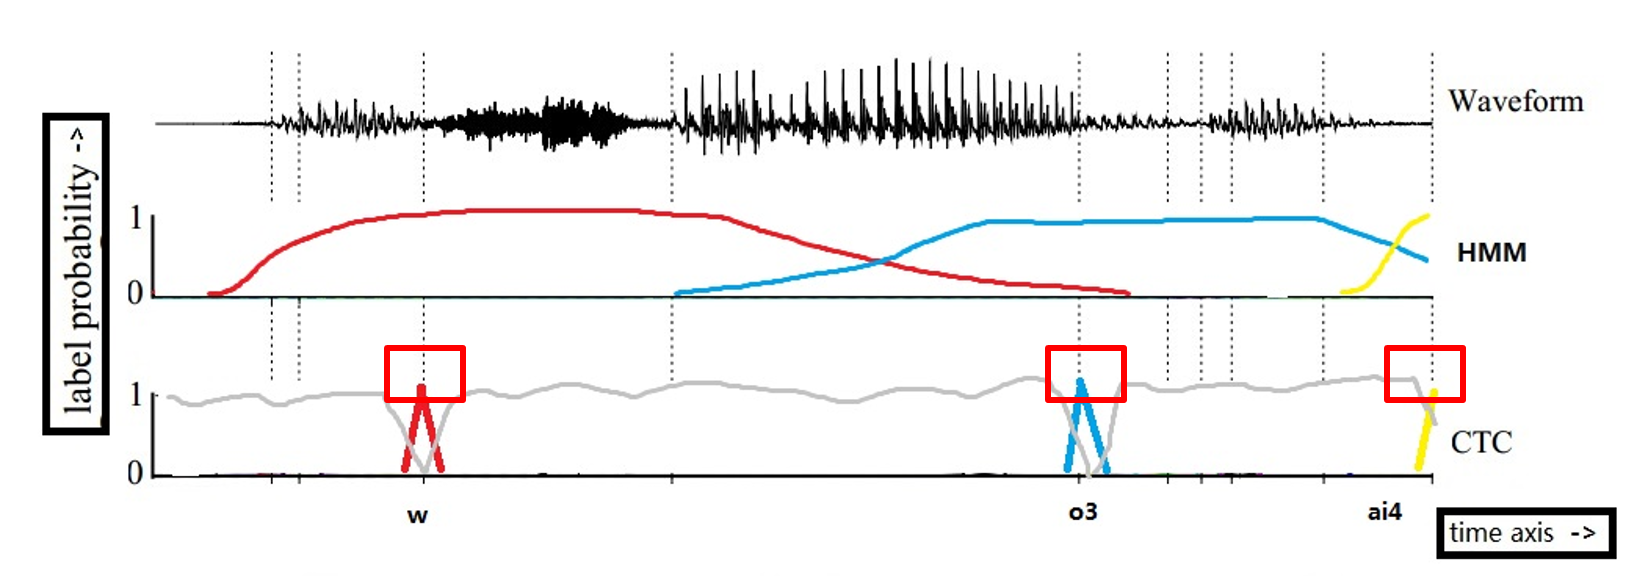
\includegraphics[width=\textwidth]{figure/peaky_distribution.png}
    \bicaption[fig:peaky-dist]{HMM,CTC的模型输出分布示例}{HMM,CTC的模型输出分布示例。纵轴表示模型输出概率,横轴表示时间。灰色分布表示CTC模型的$\tt blank$概率输出}{Fig}{The inference distributions of HMM and CTC models.}
\end{figure}

在音素级的$P(l|\mathbf{x})$的计算过程中,本文提出在帧级神经网络的输出上进行一步后处理,以便滤除$\tt blank$输出,仅保留非$\tt blank$的音素输出概率来进行公式(\ref{eq:ctc-dec-lsd})的解码搜索。本文定义公共$\tt blank$帧的集合如下:
  \begin{equation} \label{eq:com-blk-idx}
    U=\{u:y^{u}_{\tt{blank}} > \mathcal{T}\}
%    u \triangleq \left\{
%    \begin{aligned}
%    \pi\in \{\mathcal{B}(\pi_{1\mathord{:}t})=\mathbf{l}_\mathbf{w} \} \\
%    \forall \pi_u=blank
%    \end{aligned}
%    \right.
    \end{equation}


其中$y^{u}_{\tt{blank}}$ 是神经网络在第 $u$ 帧输出$\tt blank$单元的概率。在CTC模型中的softmax层,如果blank单元的声学得分足够大且接近常数1,则可以认为所有竞争路径共享相同跨度的$\tt blank$帧。 因此,忽略这些帧的分数并不会影响解码中的声学得分排序。
  \begin{equation} \label{eq:viterbi-blk-ctc}
  \begin{split}
      P(l|\mathbf{x})
      =\sum_{\pi\in\mathcal{B}(\mathbf{l})}
          \ \prod_{\pi}P(\pi|\mathbf{x})\\
      %TODO pi
        \simeq\sum_{\pi\in\mathcal{B}(\mathbf{l})}
         \  \prod_{\pi\in U}{y_{b_l}^u}{\prod_{\pi\not\in U}{y_{p_l}^u}}
        %\\ 
%        =
        %\sum_{\pi:\pi \in L',\mathcal{B}(\pi_{1\mathord{:}T})=l}
           %{\prod_{\pi\not\in U}{P(\pi|\mathbf{x})}}{\prod_{\pi\in U}{P(\pi|\mathbf{x})}}\\
%           \simeq 
                   %\sum_{\pi:\pi \in L',\mathcal{B}(\pi_{1\mathord{:}T})=l}
           %{\prod_{\pi\not\in U}{P(p|\mathbf{x})}}{\prod_{\pi\in U}{P(b|\mathbf{x})}}
        \end{split}
       \end{equation}


由于$\prod_{\pi\in U}{y_{b_l}^u}\simeq 1$,公式\ref{eq:viterbi-blk-ctc}可被推导为\ref{eq:viterbi-blk-ctc-sim}:
  \begin{equation} \label{eq:viterbi-blk-ctc-sim}
  \begin{split}
      P(l|\mathbf{x})
      %TODO pi
        \simeq\sum_{\pi\in\mathcal{B}(\mathbf{l})}
         \  {\prod_{\pi\not\in U}{y_{p_l}^u}}
        %\\ 
%        =
        %\sum_{\pi:\pi \in L',\mathcal{B}(\pi_{1\mathord{:}T})=l}
           %{\prod_{\pi\not\in U}{P(\pi|\mathbf{x})}}{\prod_{\pi\in U}{P(\pi|\mathbf{x})}}\\
%           \simeq 
                   %\sum_{\pi:\pi \in L',\mathcal{B}(\pi_{1\mathord{:}T})=l}
           %{\prod_{\pi\not\in U}{P(p|\mathbf{x})}}{\prod_{\pi\in U}{P(b|\mathbf{x})}}
        \end{split}
       \end{equation}

\subsection{标签同步解码算法实现}
\label{chap:lsd-lsd-ctc-alg}

DSM的标签同步解码算法如算法~\ref{code:lsd-dsm-alg}所示。S和E是预编译的WFST网络的起始和结束节点。Q指有效令牌,B ̂指解码路径,T是总帧数。$NNPropagate(t)$ 是每帧的声学模型推理过程。$isBlankFrame(F)$ 用于检测每帧是否为blank。 $ViterbiBeamSearch(F, Q)$是FSD中的标准维特比搜索算法,但在LSD中仅在标签级别执行。  $finalTransition(E,S,Q)$用于搜索WFST的终止节点\cite{hori2007efficient}。


\begin{algorithm}[ht]
\caption{DSM的标签同步维特比束搜索算法 \textcolor[rgb]{0,0.5,0}{(Inputs: 起始节点,结束节点,令牌队列,时间帧)}}
\label{code:lsd-dsm-alg}
\begin{algorithmic}[1]
\Procedure{ LSD for DSM } {S, E, Q, T}
\State $Q \leftarrow S$ \Comment \textcolor[rgb]{0,0.5,0}{起始节点初始化}
\For {each $t\in [1,T]$}    \Comment \textcolor[rgb]{0,0.5,0}{逐帧神经网络前向传播}
\State $F \leftarrow NNPropagate(t)$
\If {!isBlankFrame($F$)}   \Comment \textcolor[rgb]{0,0.5,0}{逐音素解码}
\State  $Q\leftarrow ViterbiBeamSearch(F, Q)$
\EndIf
\EndFor
\State $\hat B\leftarrow finalTransition(E,S,Q)$ \Comment \textcolor[rgb]{0,0.5,0}{到达结束节点}
\State backtrace($\hat B$)
\EndProcedure
\end{algorithmic}
\end{algorithm}


\section{基于无词图鉴别性训练的模型的标签同步解码}
\label{chap:lsd-lfmmi}

\subsection{标签同步解码}
\label{chap:lsd-lsd-hmm}

在GSM中,相邻HMM之间的输出标签也是条件独立的:
\begin{equation} \label{eq:viterbi-blk-hmm}
  \begin{split}
        P(\mathbf{x}|\mathbf{l}) 
        = \prod_{l} P(\mathbf{x}|l) \end{split}
       \end{equation}

类似地,在标签级别上进行的维特比搜索如下所示。
\begin{equation} \label{eq:gsm-dec-lsd}
   \mathbf{w}^* = \mathop{\arg\!\max}\limits_\mathbf{w} \left\{
        P(\mathbf{w})
        \mathop{\max}\limits_{\mathbf{l}_\mathbf{w}}  \prod_{l\in\mathbf{l}_\mathbf{w}} P(\mathbf{x}|l)\right\}
     \end{equation}

在标签中, $P(\mathbf{x}|l)$ 的计算如下所示:
\begin{equation} \label{eq:viterbi-blk-gsm}
  \begin{split}
        P(\mathbf{x}|l)
        = \sum_{\pi:\pi \in L',\mathcal{A}(\pi_{1\mathord{:}T})=l}
          \ \prod_{t=1}^{T} P(\mathbf{x}|\pi_t)P(\pi_t|\pi_{t-1})\\
= \sum_{\pi:\pi \in L',\mathcal{A}(\pi_{1\mathord{:}T})=l}
          \ \prod_{t=1}^{T} P(\pi_t|\mathbf{x})\frac{P(\pi_t|\pi_{t-1})}{P(\pi_t)}
        \end{split}
       \end{equation}  

我们在第\ref{Sec:lfmmi-train}章节介绍了几种本文所扩展的HMM拓扑结构,如图~\ref{fig:hmm-topo}(c-e)。虽然在我们的实验中,这些模型的输出分布比CTC中更平滑,但DSM中提出的公式~(\ref{eq:com-blk-idx}) 和 (\ref{eq:viterbi-blk-ctc})可以被扩展到GSM。


这里提出对神经网络的输出$P(\pi_t|\mathbf{x})$ 进行后处理,其中 $\pi_t $是帧t的推理搜索模型单元。由于这些模型中的模拟blank状态,公式\ref{eq:gsm-dec-lsd}中的维特比束搜索不必包括标签输出候选序列的所有帧。因此,给出某一帧的模型推理搜索分布时,是否从维特比搜索中排除某帧的判决如下:
  \begin{equation} 
       \label{eq:com-blk-idx-gsm}
       \begin{split}
U=\{u:\sum_{l\in L}(y^{u}_{b_l}-y^{u}_{p_l})> \mathcal{T}\}
\end{split}
\end{equation}


其中 $y^{u}_{p_l}$ 是帧u处标签输出状态l的神经网络输出,$y^{u}_{b_l}$ 是对应的blank状态的输出。在第u帧是否有标签输出,是由所有blank状态与标签输出状态的概率差异的总和决定的。T是在开发集中得到的阈值。因此, $P(\mathbf{x}|l)$  的计算可以根据 $\pi\in U$与否分为如下两部分:
\begin{equation} \label{eq:viterbi-blk-hmm2}
  \begin{split}
P(\mathbf{x}|l)
\simeq\sum_{\pi:\pi \in L',\mathcal{A}(\pi_{1\mathord{:}T})=l}
         \{\   \\ %P(b_l|p_l)P(p_l|b_l)
         \prod_{\pi\not\in U}\frac{y_{b_l}^u P(b_l|\mathbf{x})}{P(b_l)} \prod_{\pi\in U}\frac{y_{p_l}^u P(p_l|\mathbf{x})}{P(p_l)}
         \}
         \end{split}
       \end{equation}   


其中第一部分是标签输出状态。在该情况下,每个标签输出均在WFST中进行维特比搜索。而另外一组的blank部分,则假设没有标签输出。不同于CTC,不同标签输出维护自己的blank状态版本。即使是blank帧,也可能包含不同的输出标签信息。因此, $\prod_{\pi\not\in U}\frac{y_{b_l}^u P(b_l|\mathbf{x})}{P(b_l)}$的分数不能被丢弃。下文提出一种高效的算法对这一项进行计算。

这里所提出的后处理可以被视为输出标签概率$P(\pi|\mathbf{x})$的近似,从而使得维特比束搜索得以在标签级别上进行。


\subsection{标签同步解码算法实现}
\label{chap:lsd-lsd-hmm-alg}

用于GSM的标签同步解码算法如算法\ref{code:lsd-gsm-alg}所示。与算法1相比,在每个blank帧中,输出序列可以包含不同的blank单元。因此对相邻的blank帧计算$\prod_{\pi\not\in U}\frac{y_{b_l}^u P(b_l|\mathbf{x})}{P(b_l)}$ 。在非blank帧中,首先将各个blank单元各自累积得到的概率得分分别添加到当前帧的所有候选序列分数中,之后再进行维特比搜索算法。


\begin{algorithm}[ht]
\caption{GSM的标签同步维特比束搜索算法\textcolor[rgb]{0,0.5,0}{(Inputs: 起始节点,结束节点,令牌队列,时间帧)}}
\label{code:lsd-gsm-alg}
\begin{algorithmic}[1]
\Procedure{ LSD for DSM } {S, E, Q, T}
\State $Q \leftarrow S$ \Comment \textcolor[rgb]{0,0.5,0}{起始节点初始化}
\For {each $t\in [1,T]$}    \Comment \textcolor[rgb]{0,0.5,0}{逐帧神经网络前向传播}
\State $F \leftarrow NNPropagate(t)$
\If {!isBlankFrame($F$)}    \Comment \textcolor[rgb]{0,0.5,0}{逐音素解码}
\State  {\color{red}{$F \leftarrow addAccumulatedBlankScore(V,F)$ }}
\State  {\color{red}{$reset(V)$ }}
\State  $Q\leftarrow ViterbiBeamSearch(F, Q)$
\Else         \Comment \textcolor[rgb]{0,0.5,0}{accumulate $\tt blank$ scores}
\State  {\color{red}{$V \leftarrow accumulateBlankScore(V,F)$ }}
\EndIf
\EndFor
\State $\hat B\leftarrow finalTransition(E,S,Q)$ \Comment \textcolor[rgb]{0,0.5,0}{到达结束节点}
\State backtrace($\hat B$)
\EndProcedure
\end{algorithmic}
\end{algorithm}


除此之外,在HMM拓扑结构方面,本文将第\ref{Sec:lfmmi-train}章节提出的图\ref{fig:hmm-topo}(d-e)所示的几种改进结构都应用在了GSM中。

本文在维特比搜索中除了使用传统的束剪枝算法\cite{forney1973viterbi}和直方图剪枝算法\cite{steinbiss1994improvements}(自适应束剪枝\cite{van1996adaptive})之外,提出了另外两种剪枝方法。 在LSD中,blank帧占总帧数的百分比与加速比成正比,而blank帧通过公式进行判定。作为束剪枝算法的变体,这里提出了基于blank帧阈值T的剪枝算法,称为blank剪枝。当阈值T固定时,推理搜索分布的尖峰属性决定了加速比,而尖峰属性显示了神经网络输出分布的置信度。在神经网络的模型训练阶段,本文又提出了基于假设剪枝的熵剪枝算法。 在文献\cite{pereyra2017regularizing}中,作者通过惩罚确定的输出分布来防止过拟合和提高神经网络的泛化能力。受这项工作的启发, 我们在LSD框架中对输出分布的熵进行了控制,作为候选序列的剪枝方法。具体来说,在模型训练中将输出分布的熵添加到负对数似然$\mathcal{L}(\theta)$中,公式如下所示:
  
\begin{equation}
\label{equ:ent-pen-model}
\begin{split}
\mathcal{L}(\theta)= - (\ p_\theta (\pi|\mathbf{x}) - \beta H(p_\theta (\pi|\mathbf{x})\ )
\end{split}
\end{equation}

其中$H(\cdot)$是输出分布 $p_\theta (\pi|\mathbf{x})$的熵,$\beta$是正比例因子。与文献\cite{pereyra2017regularizing}不同的是,基于熵剪枝算法的训练目的是最小化模型的原有训练准则以及输出分布的熵。而通常情况下,基于熵剪枝算法是基于一个已经训练好的模型对参数进行微调。在使用新的准则训练之后,LSD框架可在少量性能损失的情况下得以加速。在接下来的实验部分,本文将详细比较这四种剪枝方法。



\section{逐帧同步解码与标签同步解码的对比}
\label{chap:lsd-lsd-hmm-alg}

本文提出将特征层面的搜索过程改变为标签层面,即搜索空间是由不同历史的标签组成的,使得解码速率等于标注速率,从而小于特征速率。具体来说,所提出的LSD的解码复杂度如下:
  \begin{equation}
\label{equ:complex-lsd}
\begin{split}
\mathbb{C}_{LSD} = O (T-|U|) \cdot \mathbb{C}_{frame}
\end{split}
\end{equation}


其中空白帧的数量 $|U|$,总是接近于T。对比公式(\ref{equ:complex-fsd})和公式(\ref{equ:complex-lsd}),FSD得到了很大的加速。这里将FSD和LSD之间的主要区别总结如下:
\begin{itemize}
\item 不同的信息率。 在FSD中,声学和语言信息均在每帧进行处理,使得二者的处理速率均和声学特征的帧率相同。而在LSD中,声学信息是以声学特征的帧率进行处理的,而语言信息则按声学模型推理的标注速率进行处理。声学和语言信息处理的不同速率去除了大量的搜索冗余。
\item 可调整的搜索间隔。 在FSD框架下,WFST网络是以等间隔遍历的(即使带有跳帧的深度神经网络在解码\cite{vanhoucke2013multiframe}时是以更长的间隔遍历语言搜索空间,但其间隔仍然是相等的)。 而在LSD中,搜索间隔可通过灵活的自我调整(在不造成性能下降的前提下)来去除blank帧带来的语言搜索空间搜索冗余,这给解码带来了很大的效率提升。
\end{itemize}


\section{实验结果}
\label{chap:lsd-exp}

本文实验使用300小时的英语Switchboard数据集作为训练数据\cite{godfrey1992switchboard},使用NIST 2000 CTS作为测试集,对NIST 2000 CTS测试集所包含的switchboard(称为swb)和call-home(称为callhm)两个子集分别进行了评估。在所有实验中使用的是经过工程优化的标准WFST解码器;实验过程中没有生成词图,也没有使用语言模型重打分~\cite{povey2012generating}技术。解码过程中使用在Switchboard和Fisher转录文本上训练的插值的4阶语言模型;在DSM算法验证中,默认使用了经过剪枝的3阶语言模型;在GSM算法验证中,默认使用4阶语言模型,使得结果与文献~\cite{povey2016purely}具有可比性。解码使用的机器配置为Intel(R)Xeon(R)CPU E5-2690 v2 @ 3.00GHz。

本文的DSM实验中,使用具有1.2 M参数的小型CTC模型,使得其适用于嵌入式设备,与文献 \cite{mcgraw2016personalized}可比;使用40维的对数滤波器组特征,特征提取窗宽为25 ms,帧移为10 ms;使用46个单音素作为声学建模单元;声学模型使用3层带有投影层的长短时记忆网络,每层包括400个节点并通过投影层压缩为128个节点~\cite{sak2014long};使用EESEN \cite{miao2016ctc}作为训练工具,训练过程与文献~\cite{miao2015eesen}相似。

本文的GSM实验是在一系列由KALDI流程\cite{povey2011kaldi}训练的基于HMM的大型模型上进行的,这些模型均适用于服务器应用。声学模型建模单元是上下文相关音素。为了提升解码性能~\cite{pundak2016lower,povey2016purely},相对于输入层特征10 ms每帧的帧率,将输出层的输出帧率下降到30 ms每帧。声学模型分别使用每层625个节点的7层时延神经网络(TDNN);以及3层带有投影层的双向长短时记忆网络(BLSTM),其中每层的前向后向层均具有1024个节点,并通过投影层压缩为256个节点。

本文的模块化训练策略的基线系统是一个无模块化训练的端到端系统,也即直接的声学到词语CTC模型,类似于~\cite{audhkhasi2017direct}, 它使用与音素CTC相同的架构,除了在输出层上使用了 30K 大小的词表作为推理搜索单元。它使用了音素CTC进行初始化。

本文实验过程中,使用词错误率(word error rate, WER)来评估不同解码框架下的模型性能,使用搜索过程中的实时率(real time factor (RTF) of the search process, SRTF)和每帧中的活动令牌的平均数量(active tokens, \#AT)来评价搜索速度。在降低帧率的声学模型中,\#AT使用降帧率之前的帧数进行计算;SRTF指解码时间与音频时间的百分比。值得注意的是,这里的解码时间不包括神经网络传播的时间\cite{you2009parallel,hauswald2015sirius}。本文所提出的框架主要加速搜索过程而非神经网络传播,因此不针对不同声学模型的计算速度进行比较,同时这里采用SRTF而不是RTF来评价搜索速度。由于在维特比搜索的搜索迭代过程-即令牌传递算法~\cite{hori2013speech}中,搜索迭代速度与有效令牌的数量相关,因此搜索速度评价指标AT与SRTF总是正相关。为了更加清晰地对比结果,我们还提供了上述指标的相对变化率($\Delta$)作为参考。

\subsection{DSM实验}
\label{exp:dsm}

(1)加速:表1给出了CTC模型下,LSD系统相对FSD系统的加速对比。基于FSD的CTC模型是基线系统。在我们的这项工作中\cite{7736093}曾进一步对比了CTC模型的性能和基于HMM的系统的性能。


\begin{table}[thbp!]
  \caption{\label{tab:exp-lsd-fsd-dsm} {\it LSD versus FSD in DSM}}
  \centerline{
  \begin{tabular}{ m{0.1\columnwidth} ||m {0.08\columnwidth} m {0.08\columnwidth} |m {0.08\columnwidth} m {0.08\columnwidth} m {0.08\columnwidth} m {0.08\columnwidth}}
\toprule
\multirow{3}{0.1\columnwidth}{测试子集  }  &
\multicolumn{2}{c|}{解码性能   }& 
\multicolumn{4}{c}{搜索加速} 
\\
&\multicolumn{2}{c|}{FSD$\mapsto$LSD}&\multicolumn{2}{c}{FSD$\mapsto$LSD}&\multicolumn{2}{c}{FSD$\mapsto$LSD}\\
&WER&$\Delta$(\%)&SRTF&$\Delta$(\%)&\#AT&$\Delta$(\%)\\
\midrule
% https://spetechcular.com/trac/aid201501/wiki/20161011lfmmi-research#modifyHMM
\multirow{1}{0.15\columnwidth}{swb} &  18.7 &+0.5&0.075&-71&2221&-77  \\
%\hline\hline
\multirow{1}{0.15\columnwidth}{callhm} &  33.3 &+0.0&0.073&-70&2211&-77 \\
\bottomrule
\end{tabular}
  }
\end{table}

swb测试子集中,在词错误率相对损失不到0.5\%的情况下,与FSD框架相比,LSD框架实现了相对70\%以上的SRTF下降(也就是3.4倍的解码加速)。解码加速主要来自于解码过程中减少了搜索迭代次数,解码过程中的活动令牌的数量也体现了这一结果。同时在callhm子集的实验中也能观察到一致的加速效果。

(2)速度鲁棒性:上面的实验解码过程中都使用一个中等大小的语言模型(3阶,3.1 M语言模型),为了测试LSD框架相对于FSD加速效果的鲁棒性(也即对复杂的语言搜索空间下的可扩展性),如图2所示,这里将解码语言模型从2阶变大到4阶[ ],大小从0.2 M变大到4.7 M,使用每帧中的平均活动令牌数(\#AT)来评价解码速度。从图 ~\ref{fig:ctc-dnn-lm-scaleup} 中可以看出,随着语言模型的增大,LSD的\#AT值几乎没有变化,而与此同时,FSD的 \#AT值则明显加速增长。此外,FSD的\#AT值总是远远超过LSD的\#AT值。也就是说,LSD实现的加速对LM搜索空间的增加是鲁棒的,GSM的实验也得出了类似的结论,因此LSD适合应用于更复杂的LM。
 

\begin{figure}[!htp]
  \centering
    \captionstyle{\centering}
    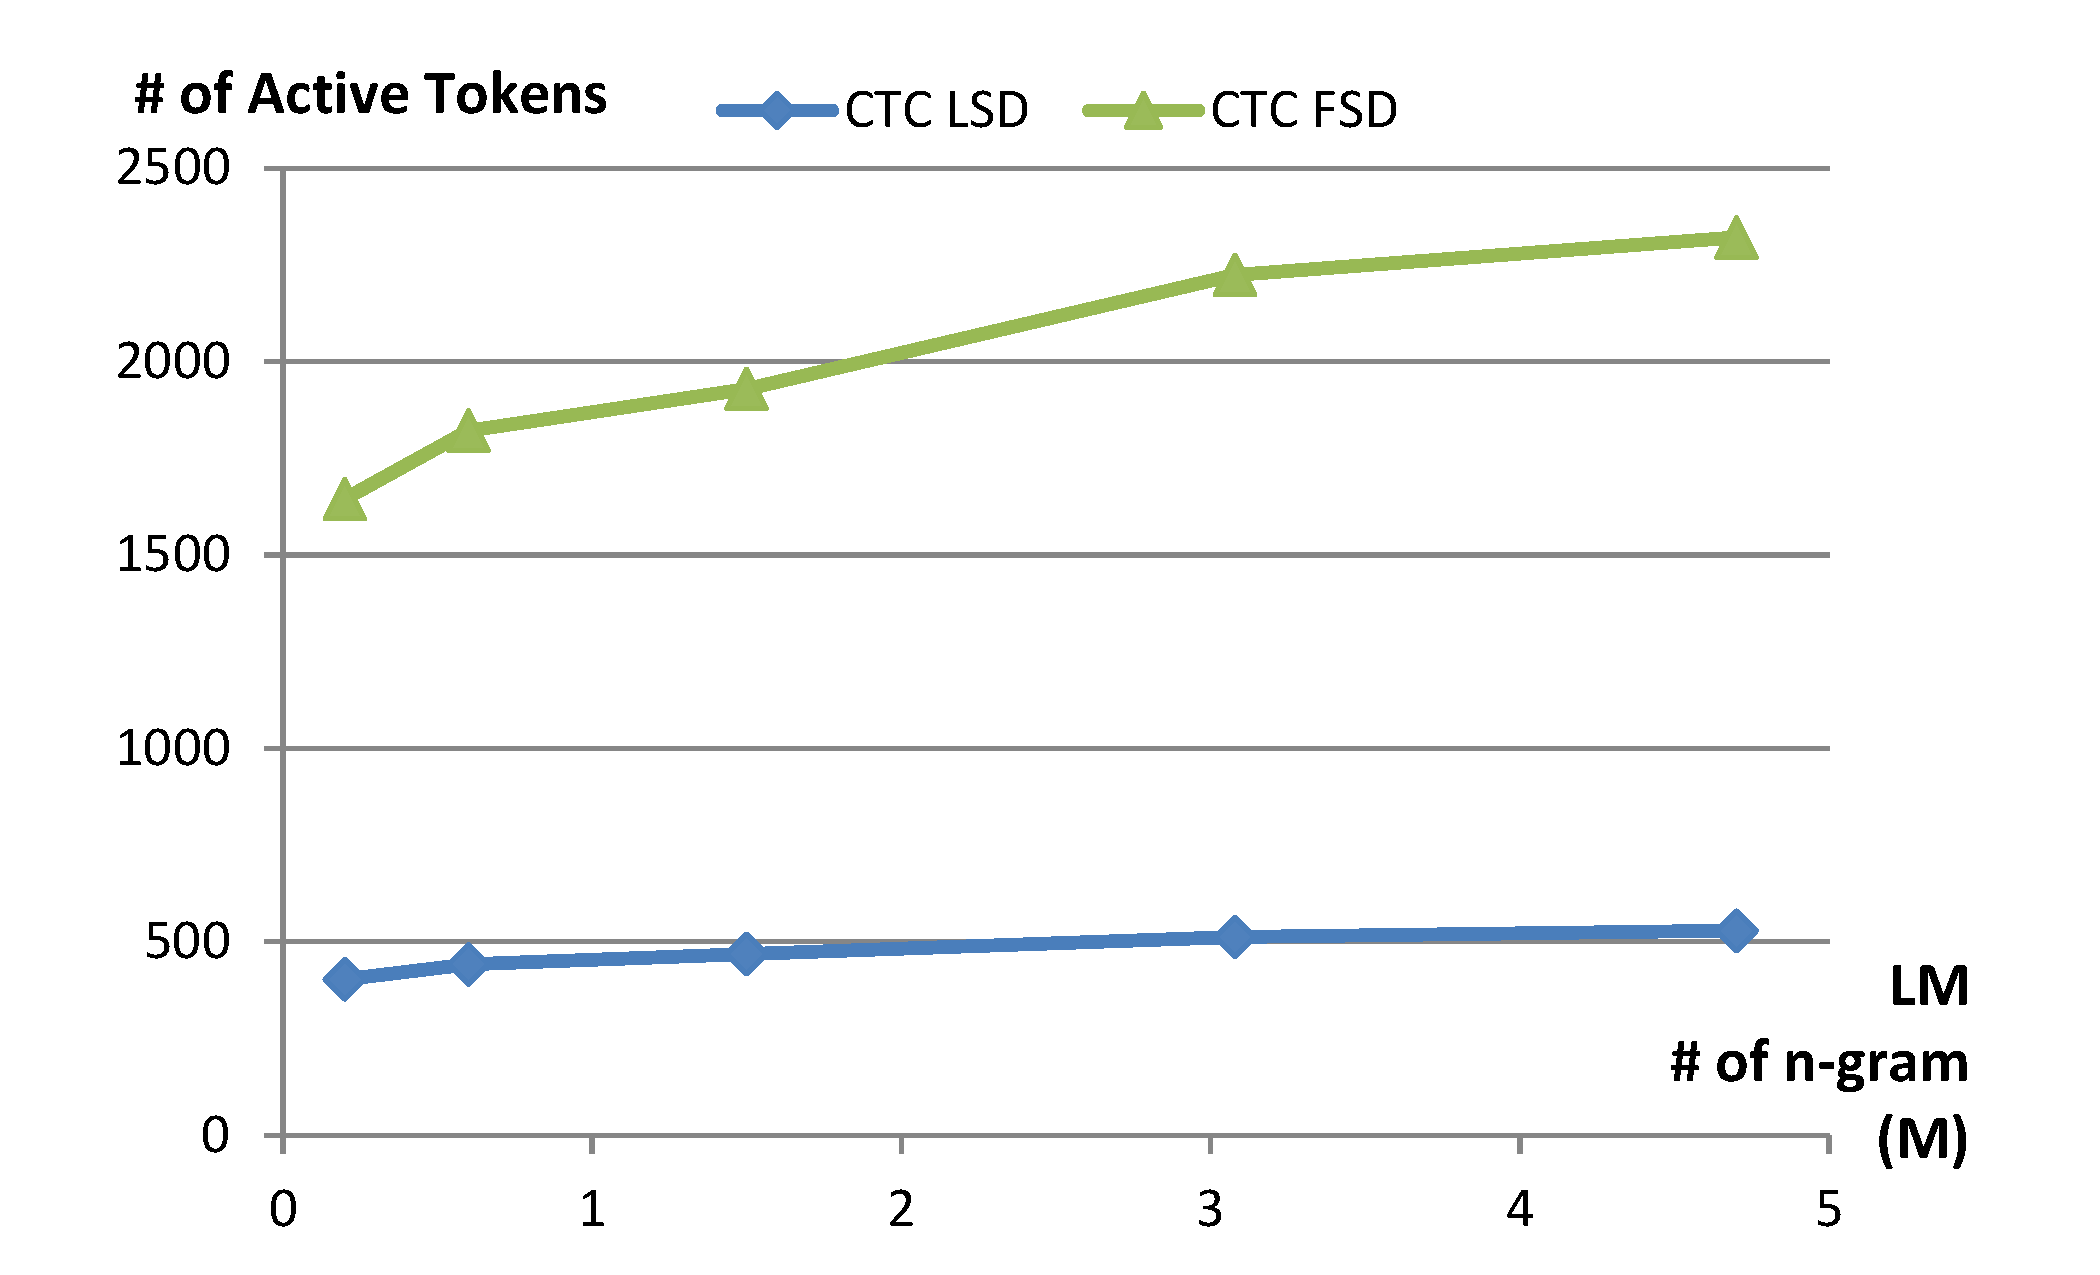
\includegraphics[width=\textwidth]{figure/speed-robust.pdf}
    \bicaption[fig:ctc-dnn-lm-scaleup]{LSD和FSD框架中平均活跃令牌数随LM变大的变化趋势}{LSD和FSD框架中平均活跃令牌数随LM变大的变化趋势。为清晰起见,这里仅绘制swb子集,calhm子集具有类似变化趋势。}{Fig}{The trend of average active token numbers and the sizes of LMs in LSD and FSD based frameworks.}
\end{figure}


(3)结合跳帧方法:该部分对比了跳帧方法下的LSD与FSD框架,实现结果表明可以将跳帧方法与FSD框架进行结合使用。值得注意的是,在后面的实验中,LSD也可以应用于跳帧或降低帧率的GSM声学模型中。

跳帧的实现方法类似于文献\cite{miao2016simplifying},这里使用LSTM-CTC的2倍跳帧(FS),并且在神经网络后验概率输出层上没有根据原始特征帧率补全后验概率,因此FS也可以加速解码过程。该方法在没有性能损失的情况下,应用于CTC模型的FS可以获得近2倍的解码性能加速。这与文献~\cite{pundak2016lower}中的观察结果一致,并且在LSTM-HMM\cite{miao2016simplifying}和DNN-HMM\cite{vanhoucke2013multiframe}也有类似的结果。LSD可以进一步与FS组合,并且获得更高的效率,即在搜索过程中进一步减少57\%(累计为78\%)的时间。


\begin{table}[thbp!]
  \caption{\label{tab:exp-cmp-vfr-lsd-dsm} {\it LSD与跳帧方法的对比}}
  \centerline{
  \begin{tabular}{ m{0.1\columnwidth} ||m {0.08\columnwidth} m {0.08\columnwidth} |m {0.08\columnwidth}  m {0.08\columnwidth} m {0.20\columnwidth} }
\toprule
\multirow{3}{0.1\columnwidth}{测试子集}  &
\multicolumn{2}{c|}{解码性能  }& 
\multicolumn{3}{c}{搜索加速} 
\\
&\multicolumn{2}{c|}{FSD$\mapsto$FS+LSD}&\multicolumn{3}{c}{FSD$\mapsto$FS$\mapsto$FS+LSD}\\
&WER&$\Delta$(\%)&SRTF&$\Delta_{FS}$&$\Delta_{+LSD} $ ($\sum$)\\
\midrule
% https://spetechcular.com/trac/aid201501/wiki/20161011lfmmi-research#modifyHMM
\multirow{1}{0.15\columnwidth}{swb} &  18.7 &-1.6&0.075&-48&-57 (-78)  \\
\multirow{1}{0.15\columnwidth}{callhm} &  33.3 &-0.6&0.073&-47&-57 (-77) \\
\bottomrule
\end{tabular}
  }
\end{table}

(4)候选序列剪枝:图\ref{fig:prune-wer-at-dsm}比较了本文提出的LSD框架与传统的剪枝技术,即束剪枝(表示为beam)和直方图剪枝(表示为histogram)。 在LSD中,通过调整公式\ref{eq:com-blk-idx}和\ref{eq:com-blk-idx-gsm}中定义的T来调整加速比和性能,这也可以被视为另一种候选序列剪枝方法(表示为blank)。 上文中提出的基于熵剪枝算法表示为entropy。
 

\begin{figure}[!htp]
  \centering
    \captionstyle{\centering}
    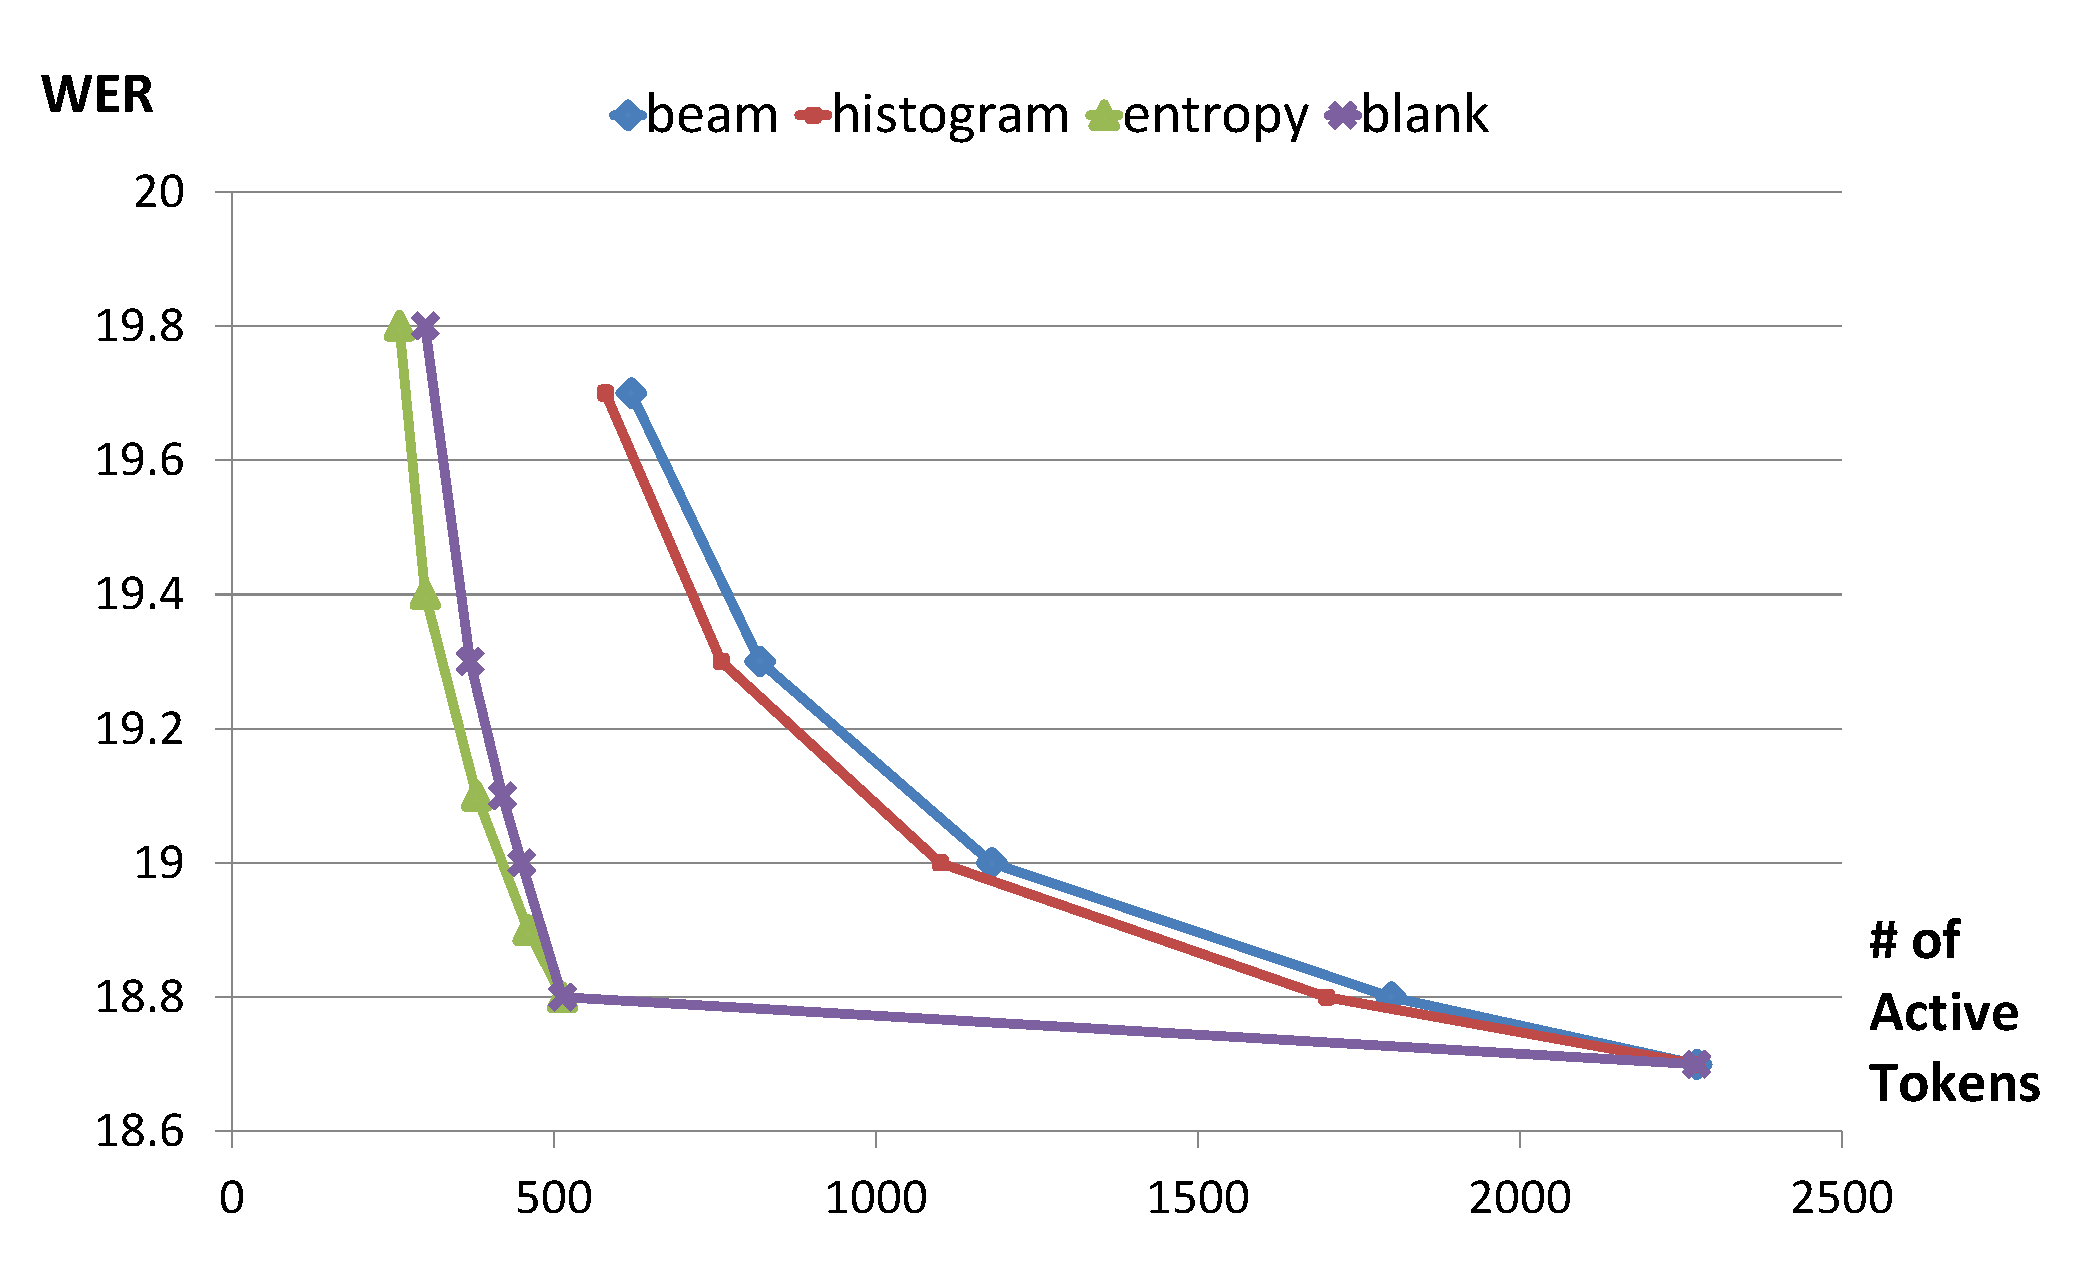
\includegraphics[width=\textwidth]{figure/prune-wer-at-dsm.pdf}
    \bicaption[fig:prune-wer-at-dsm]{swb子集,CTC中,使用不同剪枝技术时WER随平均活跃令牌数的变化趋势}{swb子集,CTC中,使用不同剪枝技术时WER随平均活跃令牌数的变化趋势。calhm子集结果类似}{Fig}{The trend of WER v.s. the number of active tokens using different pruning methods in CTC and swb-subset.}
\end{figure}


从图中可以看出,基于LSD的方法,entropy和blank,与基于FSD的方法beam和histogram相比保持显著优势。其原因在于,基于FSD的候选序列剪枝对所有候选序列进行统一处理,而相反,LSD框架可以看作是将候选序列划分为特征级别和标签级别。因此,如公式\ref{eq:ctc-dec-lsd}及公式\ref{eq:com-blk-idx}所示,LSD框架中,可以在特征层和标签层进行剪枝。也即,基于LSD的候选序列剪枝方法受益于将搜索过程从特征层转移到标签层。

另外结果显示,为了加速解码,两种框架中的方法都会降低解码性能,而且基于LSD的方法解码性能下降更严重。如前所述,基于FSD和LSD的方法之间的关键区别在于后者的阈值T仅与特征层上的候选序列剪枝有关。特征层候选序列剪枝的加速比几乎是固定的,在不损害性能的情况下,70-80\%的候选序列可以被剪枝掉。图\ref{fig:prune-wer-at-dsm}中blank曲线具有明显的拐点(\#AT = 513,WER = 18.8),也源于同样的原因。在图的最右侧,未进行特征层剪枝时,blank曲线最终达到了与基于FSD的方法的同一点。由于上面讨论的明显拐点及固定加速比,可以很容易得到等式\ref{eq:ctc-dec-lsd}中的阈值T。此外,特征层的entropy和blank剪枝可以进一步与标签层的beam和histogram方法相结合,以得到最佳的解码加速效果。为了使对比更加清晰,图中没有给出融合系统的曲线。

最后,entropy的效率略高于blank(相对约10\%)。我们认为原因在于神经网络中剪枝能更好地利用神经网络输出分布中的信息,并且产生更好的精度和效率。而blank剪枝则仅利用了输出分布中的最佳分数而未使用整个分布的信息。

\subsection{GSM实验}
\label{exp:gsm}
(1)在各种模型和准则中的应用:LSD应用于生成式序列模型(GSM)时,本文使用了多种不同的神经网络模型结构和模型训练准则进行对比;默认使用上下文相关的音素作为模型建模单元。表\ref{tab:exp-lsd-fsd-gsm}给出了在NIST 2000 CTS测试集合上的结果。总体而言,LSD框架也可以取得比较显著的解码加速,但是与表\ref{tab:exp-lsd-fsd-dsm}中的结果相比,解码加速性能变差。这是因为FSD基线的帧率已经降低到原来的1/3\cite{pundak2016lower}(类似前文中帧率改变技术可以与提出的LSD框架结合)。而且与表\ref{tab:exp-cmp-vfr-lsd-dsm}相比,加速比也略小,原因是这些模型的推理搜索分布概率不像CTC那样尖锐。如何在GSM中获取更尖锐的推理搜索分布概率将在后续章节中进行讨论。

具体地,如表~\ref{tab:exp-lsd-fsd-gsm}所示,第一行列出了文献\cite{pundak2016lower}中提出的低帧率模型(LFR)的结果;第二行是使用LF-MMI准则\cite{povey2016purely}训练出来的结果,显示出比LFR更快的搜索速度;此外,还可以看到从FSD到LSD,基于 LF-MMI准则训练的模型可以取得更快的加速。与文献\cite{paulik2015improvements}中观察到的类似,这都源于序列区分性训练准则得到的模型相对于交叉熵准则训练的模型有更尖锐的输出概率分布。第三行表示为+ sMBR,是在LF-MMI模型的基础上,使用基于LM的sMBR准则微调模型参数得到的结果;第四、五行列出了基于增强的MMI\cite{povey2008boosted}及sMBR准则变体的无需词图的区分性训练准则取得的结果,分别表示为LF-bMMI和LF-sMBR。可以观察到,本文提出的LSD框架在以上模型和准则中可以取得一致的解码加速。另外我们还使用了BLSTM模型,也都取得了相似结果。


     \begin{table}[thbp!]
        \caption{\label{tab:exp-lsd-fsd-gsm} {\it  LSD与FSD在不同的GSM模型上的性能和速度比较}}
        \centerline{
\begin{tabular}{ m{0.1\columnwidth} |m {0.15\columnwidth} ||m {0.06\columnwidth} m {0.06\columnwidth} |m {0.06\columnwidth} m {0.06\columnwidth} m {0.06\columnwidth} m {0.06\columnwidth}}
      \toprule
      \multirow{3}{0.1\columnwidth}{模型}  &
      \multirow{3}{0.15\columnwidth}{准则} & 
      \multicolumn{2}{c|}{性能 }& 
      \multicolumn{4}{c}{速度} 
      \\
      &&\multicolumn{2}{c|}{FSD$\mapsto$LSD}&\multicolumn{2}{c}{FSD$\mapsto$LSD}&\multicolumn{2}{c}{FSD$\mapsto$LSD}\\
      &&WER&$\Delta$(\%)&SRTF&$\Delta$(\%)&\#AT&$\Delta$(\%)\\
      \midrule
      \multirow{6}{0.1\columnwidth}{TDNN} & CE  & 17.8&+1.0&0.16&-38&3705&-41 \\
      & LF-MMI &15.6 &+1.0&0.13&-43 &  3386&-45\\
      %local/chain/compare_wer_general.sh tdnn_7h_sp_smbr
      & \ \ +sMBR &15.4 &+1.0&0.12&-41 & 3295 & -43 \\
      %\cline{2-5} local/chain/compare_wer_general.sh tdnn_7h_b0.1_s1_1_sp
      & LF-bMMI &15.0 &+1.0&0.11&-42 & 3198 & -44 \\
      %\cline{2-5}
      & LF-sMBR &15.3 &+1.0&0.12&-41 & 3288 & -44 \\
      \midrule
      %local/chain/compare_wer_general.sh blstm_6h_sp
      \multirow{2}{0.1\columnwidth}{BLSTM}& LF-MMI &15.2 &+1.0&0.12&-44&3290 &-47 \\
      %local/chain/compare_wer_general.sh blstm_6h_b0.2_s2_3_sp
      & LF-bMMI &14.3 &+1.0&0.11&-43& 3205&-45 \\
      \bottomrule
      %\hline\hline
      \end{tabular}
        }
      \end{table}



(2)候选序列剪枝:如图\ref{fig:prune-wer-at-gsm}所示,我们在生成式序列模型下进行了一系列候选序列剪枝相关的实验,其变化趋势类似于DSM中的结果,读者可以参考那里的讨论。与图\ref{fig:prune-wer-at-dsm}中一个区别在于,beam,histogram,blank,entropy在图\ref{fig:prune-wer-at-gsm}中的最左边位于相同点,这表明在降低帧率的情况下,特征层候选序列剪枝的最大比例较小。 然而,在解码性能的WER达到最佳时,仍然有接近两倍的解码加速。



\begin{figure}[!htp]
  \centering
    \captionstyle{\centering}
    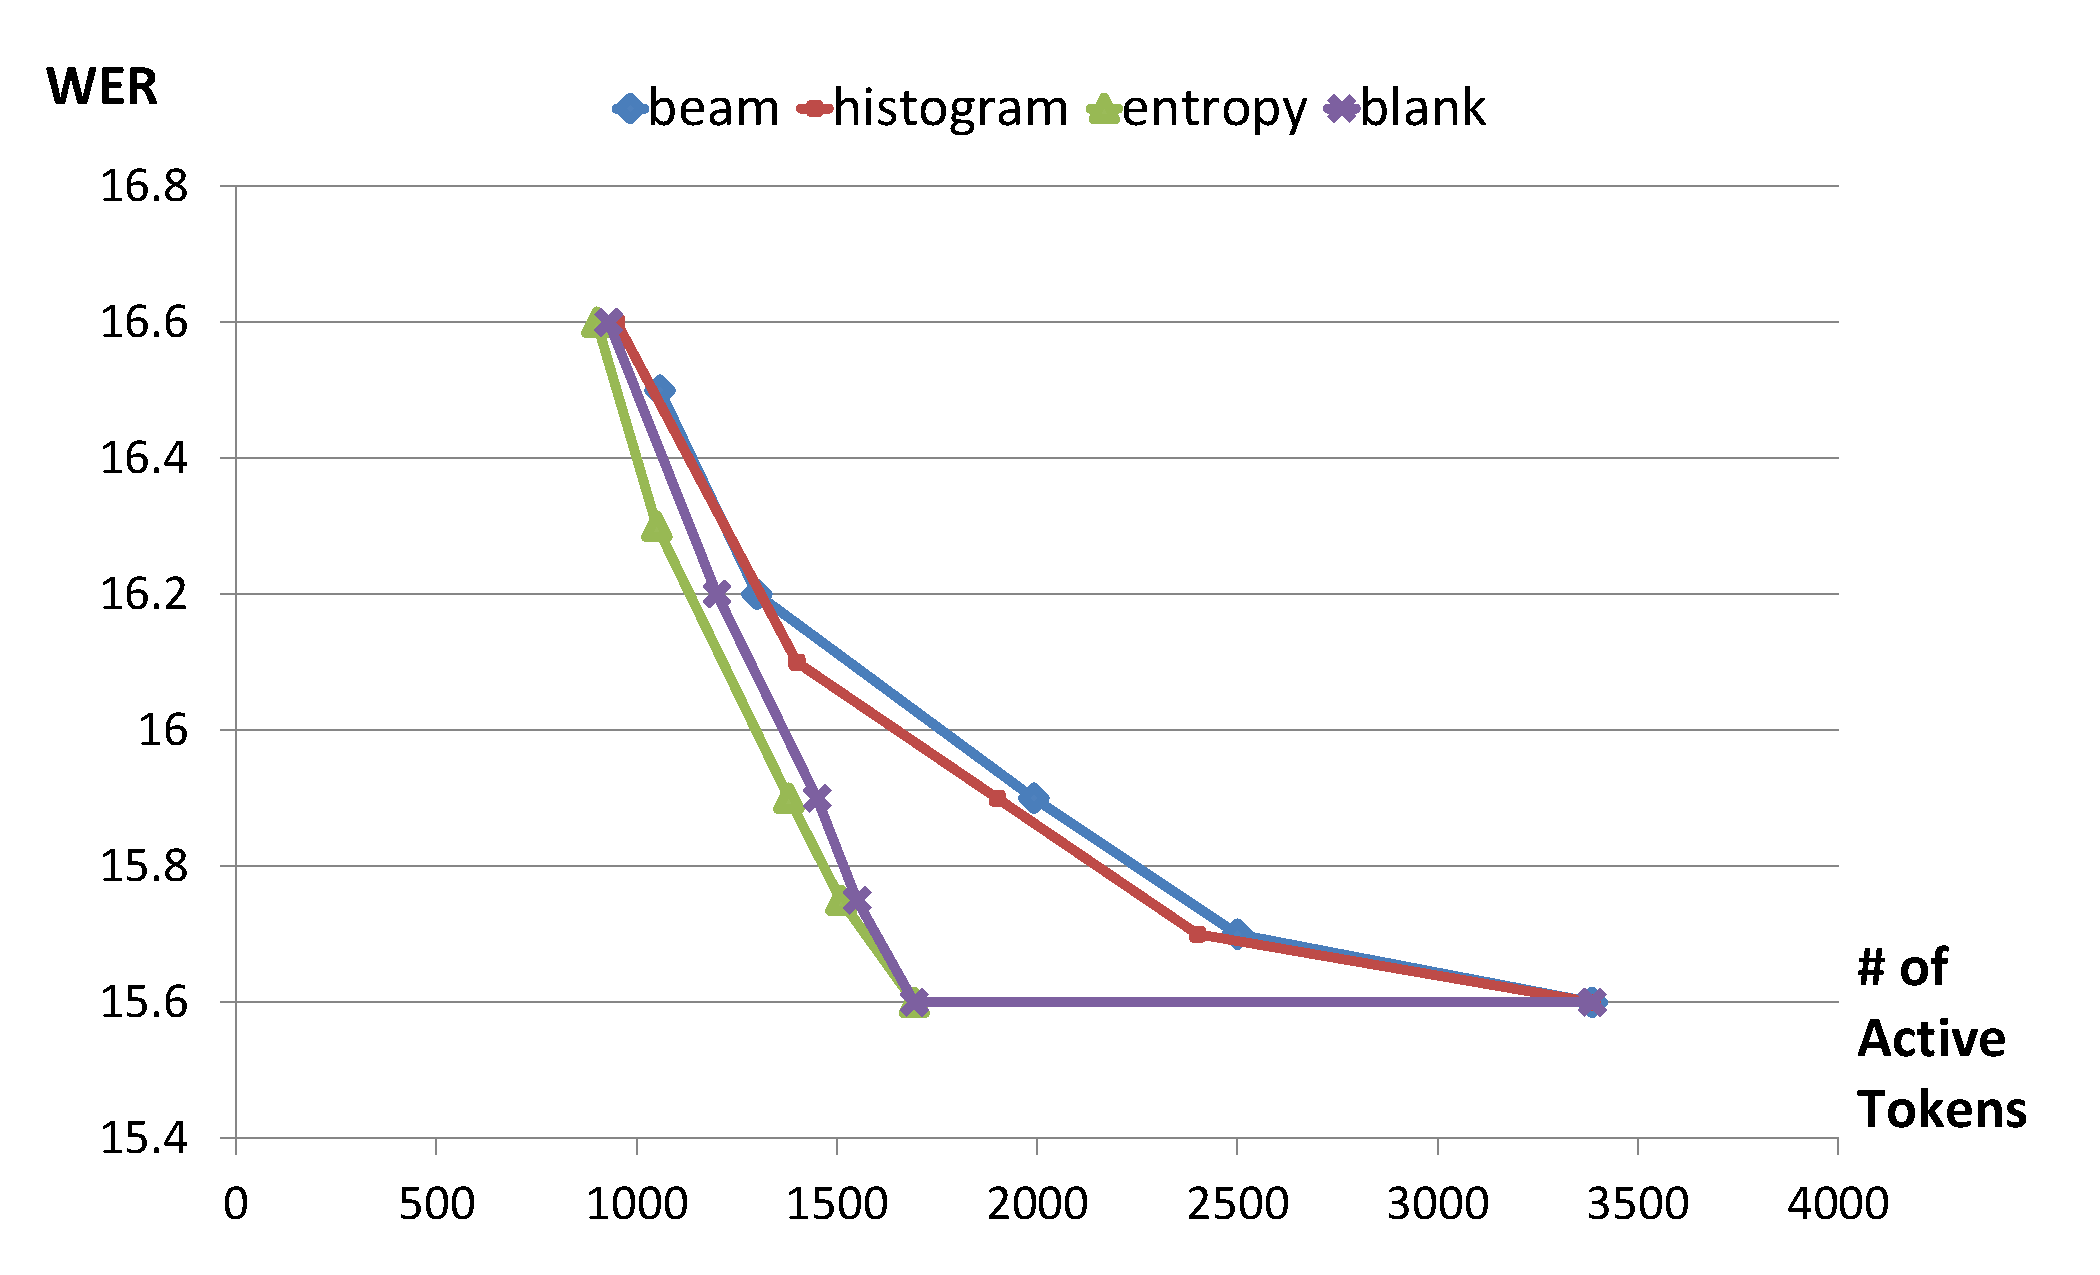
\includegraphics[width=\textwidth]{figure/prune-wer-at-gsm.pdf}
    \bicaption[fig:prune-wer-at-gsm]{LF-MMI中,使用不同剪枝技术时WER随平均活跃令牌数的变化趋势}{LF-MMI中,使用不同剪枝技术时WER随平均活跃令牌数的变化趋势}{Fig}{The trend of WER v.s. the number of active tokens using different pruning methods in LF-MMI.}
\end{figure}

   
(3)进一步设计:本节将对比前文中讨论的各种转移模型,以及由此获得的效率的进一步提高。该部分所有实验均在LF-MMI准则上进行,但实验结论可以扩展到其它神经网络和训练准则上。 


     \begin{table}[thbp!]
        \caption{\label{tab:exp-blk-gran-gsm} {\it 生成式序列模型中的blank粒度}}
        \centerline{
    \begin{tabular}{ m{0.1\columnwidth} |m {0.15\columnwidth} ||m {0.06\columnwidth} m {0.06\columnwidth} |m {0.06\columnwidth} m {0.06\columnwidth} m {0.06\columnwidth} m {0.06\columnwidth}}
      \toprule
      \multirow{3}{0.1\columnwidth}{系统}  &
      \multirow{3}{0.15\columnwidth}{$\tt blank$} & 
      \multicolumn{2}{c|}{性能 }& 
      \multicolumn{4}{c}{速度} 
      \\
      &&\multicolumn{2}{c|}{FSD$\mapsto$LSD}&\multicolumn{2}{c}{FSD$\mapsto$LSD}&\multicolumn{2}{c}{FSD$\mapsto$LSD}\\
      &&WER&$\Delta$(\%)&SRTF&$\Delta$(\%)&\#AT&$\Delta$(\%)\\
%      \hline \hline
      %\multirow{2}{0.13\columnwidth}{CE} & $\times$ & & & \\
%      \cline{2-5}
%      & $\surd$ & & & \\
%      \hline\hline
      %\multirow{2}{0.15\columnwidth}{sMBR} & $\times$ & & & \\
%      \cline{2-5}
%      & $\surd$ & & & \\
      \midrule
      \multirow{3}{0.15\columnwidth}{TDNN LF-MMI} &  CD phone &15.6 &+1.0&0.13&-43&3386&-45 \\
      & phone &15.7 &+0.9&0.09&-47&2785& -50\\
      % local/chain/run_tdnn_7h_inphone.sh
      % ref: https://spetechcular.com/trac/asr/milestone/report-yby23-2016-11-06
      %local/chain/compare_wer_general.sh tdnn_7h_mhmm_BP_sp
      & global &16.8 &+0.8&0.09&-49&2512& -54 \\
      \bottomrule
%      \hline\hline
      \end{tabular}
        }
    \end{table}

表~\ref{tab:exp-blk-topo-gsm}中列出了不同blank粒度的对比结果,即上下文相关的音素blank (CD phone blank),音素blank (phone blank)和全局blank (global blank)。与CD phone blank基线相比,phone blank在取得近似的解码性能的同时,实现了显著的搜索过程加速;这里搜索加速主要源于较少的模型建模单元,即模型状态数从6K减少到3K。此外,从表中可以看出,global blank会带来明显的性能下降;global blank需要足够的数据来覆盖不同相邻音素之间的上下文环境(我们认为这也是CTC准则在这个语料库中表现更差的原因之一);CD phone blank可以缓解blank训练数据不足的问题,但会导致搜索速度变慢;因此,绑定中心音素相同的CD phone blank在加速搜索过程的同时,也可以更好地建模blank模型;因此,phone blank是解码性能和搜索速度之间的最佳平衡。此外,从表\ref{tab:exp-blk-topo-gsm}中可以看出,在LSD框架下,较少的模型单元可以持续带来明显的搜索过程时间缩短:从43\%到 47\%,再到 49\%。最后,phone blank是基于GSM的LSD框架的最佳选择。


     \begin{table}[thbp!]
        \caption{\label{tab:exp-blk-topo-gsm} {\it 生成式序列模型中的blank拓扑结构}}
        \centerline{
        \begin{tabular}{ m{0.1\columnwidth} |m {0.1\columnwidth} ||m {0.06\columnwidth} m {0.06\columnwidth} |m {0.06\columnwidth} m {0.06\columnwidth} m {0.06\columnwidth} m {0.06\columnwidth}}
      \toprule
      \multirow{3}{0.1\columnwidth}{测试集}  &
      \multirow{3}{0.1\columnwidth}{拓扑} & 
      \multicolumn{2}{c|}{性能 }& 
      \multicolumn{4}{c}{速度} 
      \\
      &&\multicolumn{2}{c|}{FSD$\mapsto$LSD}&\multicolumn{2}{c}{FSD$\mapsto$LSD}&\multicolumn{2}{c}{FSD$\mapsto$LSD}\\
      &&WER&$\Delta$(\%)&SRTF&$\Delta$(\%)&\#AT&$\Delta$(\%)\\
%      \hline \hline
      %\multirow{2}{0.13\columnwidth}{CE} & $\times$ & & & \\
%      \cline{2-5}
%      & $\surd$ & & & \\
%      \hline\hline
      %\multirow{2}{0.15\columnwidth}{sMBR} & $\times$ & & & \\
%      \cline{2-5}
%      & $\surd$ & & & \\
      \midrule
      % https://spetechcular.com/trac/aid201501/wiki/20161011lfmmi-research#modifyHMM
      \multirow{3}{0.15\columnwidth}{TDNN LF-MMI} &  PB &15.6 &+1.0&0.13&-43&3386&-45  \\
      & BP & 15.6 &+1.0&0.13&-46&3392&-49 \\
      %sharper than BPgB
      %& gBPB & 10.4&+1.0&&&& \\
      & BPB & 15.6 &+1.0&0.13&-47&3388&-51 \\
      \bottomrule
%      \hline\hline
      \end{tabular}
        }
    \end{table}

表\ref{tab:exp-blk-topo-gsm}对比了前文提出的不同HMM拓扑结构。在FSD框架下,所有拓扑结构都有相似的解码结果和相同的搜索速度。对比前两行可以看出,与基线PB拓扑结构相比,在LSD框架下, BP可以获得更大的搜索加速。我们认为这个更优的搜索加速源于标签延迟现象,类似于文献\cite{amodei2015deep}中观察到的现象,这使得模型能更可靠地推断标签输出状态并减少混淆。因此,这能带来更尖锐的输出分布。从表中还可以看出,BPB拓扑结构可以进一步改善搜素速度;一些解码路径的例子也表明这种拓扑结构可以使每个上下文相关的隐马尔可夫模型输出更多的blank状态。最后,与前面表中CTC的结果相比,GSM中LSD框架能减少49\%的搜索时间。


\section{本章小结}
\label{chap:lsd-sum}

在本章中,我们针对语音识别和端到端建模的推理搜索阶段,提出了标签同步解码算法,其通过一系列方法使得搜索解码过程从逐帧同步变为标签同步,这包括使用高效的blank结构和后处理方法。该文提出的一系列通用方法在隐马尔科夫模型和连接时序分类模型上得到了验证。同时该章节还介绍了将标签同步算法应用于序列到序列的端到端模型的方案。在实验部分,该章节系统取得了大幅度语音识别解码速度改善。
